\documentclass[UTF8,a4paper,11pt]{ctexart}
% \usepackage[utf8]{inputenc}
\usepackage{fontenc}
\usepackage{lmodern}
\usepackage{xeCJK}
\setCJKmainfont[BoldFont={Noto Serif SC}, ItalicFont={Noto Serif SC}]{Noto Serif SC}
\setCJKsansfont{Noto Sans SC}
\setmonofont{JuliaMono}

\usepackage{amsfonts,amssymb,unicode-math}
% \usepackage{mathtools}

%%%%%%%%%%%%%%%% 设置边距
\usepackage{geometry}
\geometry{a4paper,left=2.54cm,right=2.54cm,top=3.17cm,bottom=3.17cm}

%%%%%%%%%%%%%%%% 章节标题对齐
% \usepackage{sectsty} % 左对齐章节标题
% \sectionfont{\bfseries\Large\raggedright}

%%%%%%%%%%%%%%%% 常用的环境
\usepackage{graphicx,caption,booktabs,float,fancyhdr,enumerate}

% 算法包
% \usepackage{algorithm2e}
\usepackage{listings}
% \usepackage{minted}

% 超链接
\usepackage{hyperref}
\usepackage{url}
\usepackage{doi}

% 换页 自定义了一个命令。\newpage很多时候不管用
\newcommand*{\forcednewpage}{\newpage\null\newpage}

% 引用
\usepackage[english]{babel}
\usepackage[%
style=phys,%
articletitle=false,biblabel=brackets,%
chaptertitle=false,pageranges=false%
]{biblatex}

%% 添加引用bib
\addbibresource{ref.bib}

% 颜色
\usepackage{xcolor}
\definecolor{codebgc}{HTML}{F9F4FC}
\usepackage[most]{tcolorbox}
% \colorlet{LightLavender}{Lavender!40!}
\tcbset{on line, 
        boxsep=3pt, left=0pt, right=0pt, top=0pt, bottom=0pt,
        colframe=white, colback=codebgc,  
        highlight math style={enhanced}
        }

% inline 代码
\newcommand{\ic}[1]{\tcbox{
\texttt{\textcolor{purple}{\footnotesize{#1}}} 
}}

% \pagestyle{fancy}
% \lhead{}
% \chead{}
% \rhead{\rightmark}
% \fancyhf{}




\pagestyle{fancy}
\fancyhead[L]{{Coupled Mode Description of Applause Dynamics}}
% \chead{}
% \rhead{}
% \fancyhf{}
\graphicspath{{./figures/}}

\title{
Statistical Physics Course Project\\
\vspace{0.5em}
Coupled Mode Description of Applause Dynamics
}
\author{
张腾洲\thanks{学号:022072910045 \hspace{1em} 物理与天文学院22级}
}
\date{\today}

\begin{document}
\maketitle
\begin{abstract}
    We have proposed a nonlinear mean-field model to investigate the dynamics of applause in a crowd, utilizing the coupled mode theory (CMT). The model is numerically solved, and we apply time-frequency analysis to examine its solution. Our findings reveal a threshold effect of the initial applauding ratio, highlighting its crucial role in the dynamics. Furthermore, we verify that synchronization arises from the interplay between heterogeneity and coupling strength. Remarkably, different leading factors yield similar temporal patterns with distinctive spectral characteristics.
\end{abstract}

\newpage
\tableofcontents

\newpage

\section{Statement of the Problem}

Applause of crowds is an emergent phenomenon rather than a sum of individual behaviors. How people burst into applause and what factors may contribute to the amplitude, duration and rhythm of the applause are not yet extensively studied, as Patrick J. Kiger commented in \emph{How Applause Starts and Spreads Is Oddly Scientific}.

\subsection{Historical Investigations}

In historical investigations, there are mainly two formalisms to this problem, each with a different approach and focus.

One formalism focus on how the applause spreads and how does the intensity changes with time. It adapts compartmental models, among which the \textbf{susceptible-infected-recovered (SIR) model} and its variants, both deterministic  and are the most widely used. For a SIR based model for applause dynamics, see \cite{mann2013dynamics}; for some analytical results spatial SIR model, see \cite{PhysRevE.82.051921}.

Another formalism, whose focus mainly lies in the synchronization phenomenon during applauses, is proposed by N\'eda,\emph{et al.} in \cite{appPRE,neda2000sound}. Participants are modeled as coupled nonlinear oscillators. This kind of model for collective synchronization are also usually referred as \textbf{Kuramoto model}\cite{kuramoto1975self}.

\subsection{Aim of this Project}
In previous studies, researchers either focused solely on the propagation of applause behavior within a crowd or solely on the synchronous patterns of applause frequency. Therefore, this paper aims to propose \textbf{a unified descriptive framework for behavioral contagion, intensity variation, and synchronization phenomena during applause}, and enhancing our understanding of the following issues:

\begin{enumerate}
    \item Does a collective applause exhibit a \textbf{threshold} effect? In other words, does the initial proportion of individuals engaging in applause within a crowd influence the final intensity and duration of applause?

    \item What factors contribute to the \textbf{synchronization} of applause and how is it influenced? We especially investigate the effects of \textbf{heterogeneity (or homogeneity)}.
\end{enumerate}

\subsection{Considerations \& Criteria of a Good Model}

Before introducing the model, we first list some physical considerations for a \textbf{physical} model of applause dynamics. 

\begin{enumerate}
    \item A good model, in sense of physics, should have \textbf{as few parameters as possible} while ensuring that each parameter has a \textbf{meaningful physical interpretation}. We only propose the parameters necessary for deducing essential physical facts, whereas other parameters, even if listed, should be irrelavent to the results or just complementary to necessary parameter and can be fixed at first.
    \item \textbf{Mean-field vs spatial}: a spatial model is very appealing, however the spatial dimension is not necessary for a quanlitative model, because:
        \begin{itemize}
            \item The \textbf{reverberation effect} makes it hard to for one to distinguish the sound from different individuals during the applause. The intensity of applause heard by all audience members is essentially the same.
            \item We should not make \textbf{a prior assumption} that crowds conform to specific spatial distributions and configurations, as they can vary significantly across different scenarios.
        \end{itemize}
        Therefore we only construct a \textbf{mean field model}. The spatial version can be easily derived, but this introduces more parameters, and is contradictory to the first consideration.
    \item \text{ODE vs Stochastic}: 
        The utilization of stochastic differential equations (SDEs) or Markov processes may not necessarily capture additional information, as the dynamical system itself exhibits chaotic behavior, and uncertainty can be introduced through parameter distributions. Besides, the master equation corresponding to the Markov process is also an ordinary differential equation (ODE). Therefore, we employ ODEs to model this system, considering its chaotic nature and the introduction of uncertainty via parameter distributions.
\end{enumerate}

\section{Model \& Method}

\subsection{Coupled Mode Theory}
Coupled mode theory (CMT) is a theoretical framework used to describe and analyze the interaction between multiple modes in a waveguide or resonator system. It is commonly applied in various fields, including optics, photonics, and acoustics. For a detailed tutorial and applications, see \cite{CMT}. In coupled mode theory, the modes of a resonance system are treated as independent oscillators that can interact with each other, with a linear form:
\begin{equation}
    \frac{\mathrm{d}}{\mathrm{d} t} u_j = (iω_j-γ_j)u_j + i\sum_{k} κ_{jk}u_k,
\end{equation}
where $u_j$ is the complex mode of each resonator like variable and $ω_j,γ_j,κ$ are the intrinsic frequency, loss factor and coupling between modes, respectively. If $γ_j=0$ and $κ$ is symmetric, the equation will be nothing new but a Schrodinger equation. However, with the loss factor $γ_j$ this mode natively capture the dissipation in classical system. More generally, this equation can be nonlinear, with not only loss but gain, and needs to by expressed as:
\begin{equation}
    \frac{\mathrm{d}}{\mathrm{d} t} u_j = [iω_j + g_j(𝐮,t) - γ_j(𝐮,t)] u_j + i\sum_k κ_{jk}(𝐮,t)u_k,
\end{equation}
Which is the most general case. By solving the coupled mode equations one can determine the evolution of the modes over time. This analysis enables the prediction of phenomena originates from the interaction between modes.

CMT is a good candidate for modeling the applause dynamics, because the individuals can be treated as oscillators with both phase and amplitude, while their interactions can be parameterized as the gain/loss and coupling terms.

\subsection{Overview of the Model}

In our model, each individual is labeled by a complex mode $u_j$ and the evolution obeys the CMT equation with \textbf{two} mean-field terms:

\begin{equation}
    \begin{split}
        & \frac{\mathrm{d}}{\mathrm{d} t} u_j = \left\{ i \left[ ω_j + κ_j⋅|ϕ|\sin\left(\arg\frac{ϕ}{u_j}\right) \right] + g_j(\bar{F}(𝐮), u_j, t)  \right\} u_j,\\
        & \text{order parameter: }\,\, ϕ(t) = {⟨u_j(t)⟩}/{\sqrt{⟨|u_j(t)|^2⟩}} = \frac{\sum u_j(t) }{N||u(t)||},\\
    \end{split}
    \label{eq:cmtapp}
\end{equation}
where each parameter or function with label $j$ is unique. In eq.\ref{eq:cmtapp}:

\begin{enumerate}
    \item $u_j$ is the complex mode of each person. Note that this is \textbf{not} the applause amplitude of a person. However, $u_j$ characterize the frequency and amplitude of individual applause. $|u_j|$ has positive correlation to the amplitude $F(u_j)$.
    \item $ω_j$ is the intrinsic oscillatory frequency. This denote that, the frequency of applause for each individual, in the absence of influence from others, is a unique constant.
    \item The parameter $κ_j$ represents how likely each individual is to synchronize their applause with others. The mean field term $ϕ(t)$ is an \textbf{complex order parameter} appears as the collective rhythm. If the phase $\arg{ϕ}$ is ahead of individual and the amplitude $|ϕ|$ is not very small, he trys to catch the rhythm and increase his frequency. This can also be understanded as \textbf{an analog of Kuramoto model}.
    \item The function $g_j$ represents the enthusiasm level of individual(the gain or loss factor of the rotor), influenced by both their individual personality and the environment. The \textbf{only} parameter we consider so far is the average applause \textbf{intensity} named $\bar{F}(𝐮)$, which depend on the individual intensity $\bar{F}(𝐮) = \frac{1}{N}\sum_j F(u_j)$. This is also a mean field term. If $g_j>0$ at certain moment, the person increase the amplitude of his mode, otherwise the mode is damping. There are other parameters in $g_j$ as explained below.
\end{enumerate}

Before delving into the details of the model, we provide the following qualitative explanation of the dynamics of applause: Each individual is represented by a nonlinear rotor and makes \textbf{two} distinct contributions to the environment (\textbf{the mean field}); one contribution is related to the intensity of applause, involving only the strength aspect, while the other contribution is associated with collective oscillation modes, incorporating \textbf{phase} information. Moreover, each individual's behavior is influenced by the intensity and phase of the mean field, where the intensity component, in turn, affects the enthusiasm of each individual's applause, while the collective modes drive individuals to adjust their phases and synchronize with each other.

The detailed description for functions $g_j,F$ will  be derived in the next subsection.

\subsection{Model Details}

\subsubsection{Heterogeneity of parameters}

We must consider the variations in individual parameters. To account for this, we assume that the parameters of the population follow a Gaussian distribution. Furthermore, to mitigate the physical singularity caused by outliers, we truncate the distribution at the $1σ$ position. For one parameter $λ$, we assume that
\begin{equation}
    λ_j = \bar{λ} ⋅(1+σ_λ ξ_j),\quad ξ_j \sim \mathcal{N}(0,1),
\end{equation}
where $ξ_j$ is re-sampled if $|ξ_j| >1$. $σ_λ$ is a dimensionless variance that represents the heterogeneity.

For example, for $\bar{ω}/2π=3.0$ we get the following distribution within 1000 person as shown in Fig.\ref{fig:omegadist}.

\begin{figure}[H]
    \centering
    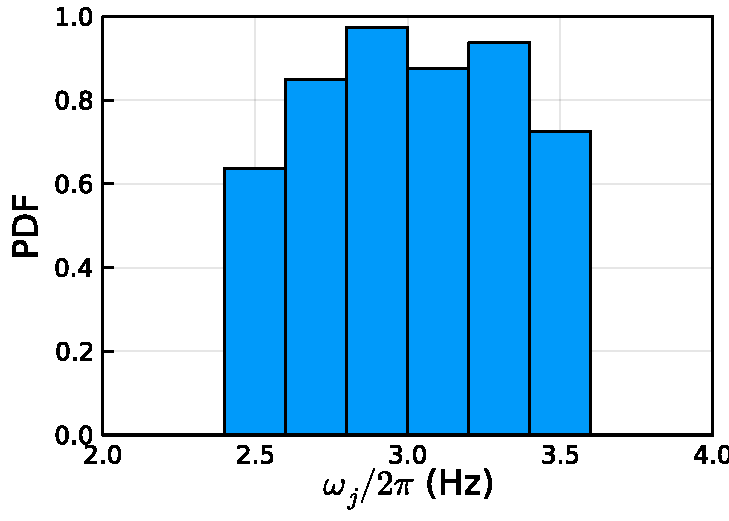
\includegraphics[scale=0.6]{omegadist.pdf}
    \caption{The clapping intensity signal series of 4 different people during a applause.}
    \label{fig:omegadist}
\end{figure}

In our investigation we take $σ_λ$ the same for all parameters $λ→ω,κ,τ...$. This is a very rough simplification, however, as we should see, that $σ_ω$ plays a very important role in synchronization, but the effect of other variances seem to be not obvious.

\subsubsection{Clapping intensity}

We model the clapping\footnote{Here we use the word ``clapping'' rather than ``applause''. The clapping is considered as the main contribution in applause.} intensity with the following function:
\begin{equation}
    F(u_j) = 2 ⋅ l(\mathrm{Re}(u_j)-1,0.1).
    \label{eq:clapfun}
\end{equation}

The basic idea is to find a peak function for a periodic input $u_j = u_0 e^{iωt}$ with a threshold for $u_0$. The form Eq.\ref{eq:clapfun} is just parameterization.

\begin{figure}[H]
    \centering
    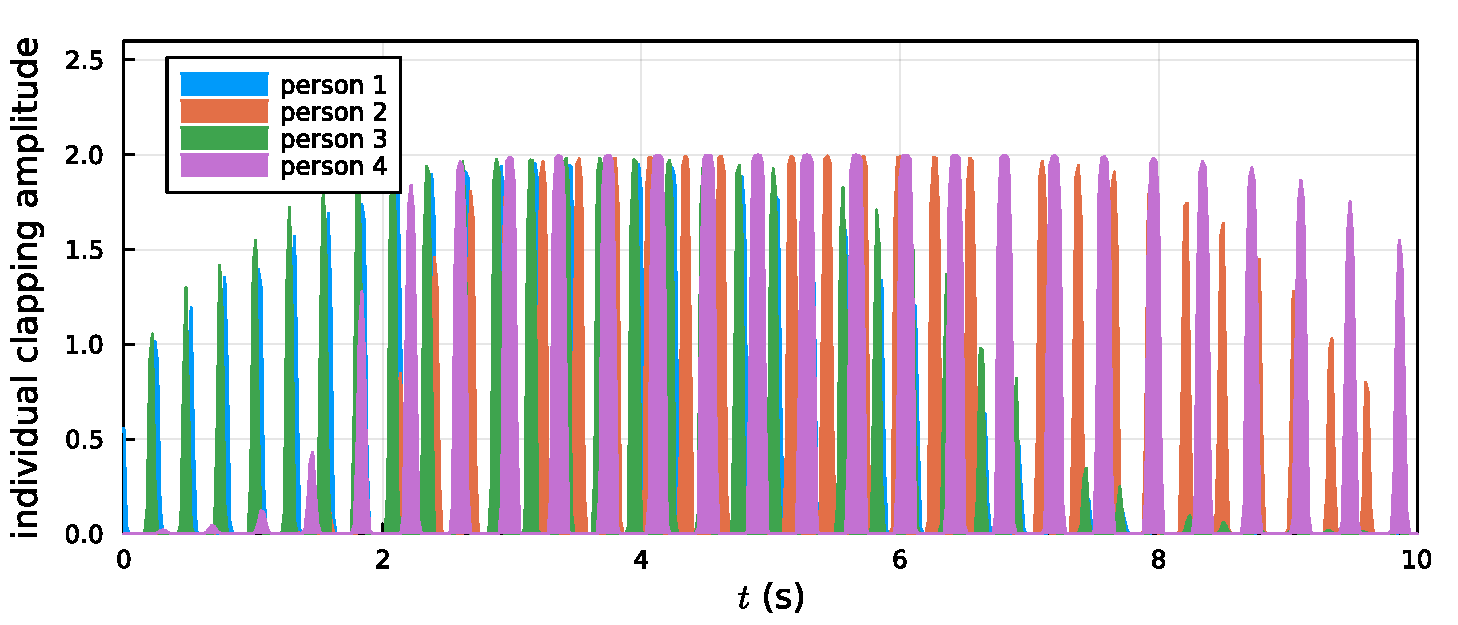
\includegraphics[scale=0.6]{individualclap.pdf}
    \caption{The clapping intensity signal series of 4 different people during a applause.}
    \label{fig:ind_clap}
\end{figure}

In order to demonstrate the effectiveness of this parameterized approach, we have selected and depicted the intensity-time relationship of applause for four different individuals from a complete simulation, as shown in Fig.\ref{fig:ind_clap}. It can be observed that the maximum intensity of the pulse is approximately 2, while the threshold is around 1. When the input mode's amplitude falls below 1, the pulse rapidly attenuates.

\subsubsection{Enthusiasm \& patience}

The gain/loss factor of individual mode is parameterized by the function
\begin{equation}
    g_j(\bar{F}, u_j, t) = g_{j0} \bar{F} (1-p_γ)(1-p_b) - p_γ γ_j,
\end{equation}
where $g_{j0}$ is a constant representing how easily is the individual inspired by others and $γ_j = τ_j^{-1}$ describes the patience of this individual. $τ_j$ is defined as the expectated duration of individual applause with the absence of others. Also
\begin{equation}
    p_γ = l(t-τ_j,1.0), \quad p_b = l(|u_j|-1,0.2),
\end{equation}
are two shaping functions. As $t>τ_j$, $p_γ$ makes the damping factor $γ_j$ dominate, and the individual tends to stop clapping regardless of the environment. while for $t<τ_j$, the enthusiasm dominates the factor and is affected by the mean intensity $\bar{F}$.

\begin{figure}[H]
    \centering
    \includegraphics[width=0.9\textwidth]{gfunc.pdf}
    \caption{The function $g_j(\bar{F},u_j,t)$ where $g_{j0}=4.0\,\mathrm{s^{-1}}$ and $τ_j=5.0 \,\mathrm{s}$. Also we take $|u_j|=1$.}
    \label{fig:gfunc}
\end{figure}

We visualize the function $g_j$ in Fig.\ref{fig:gfunc}. It can be observed that after $t≈5$ the enthusiasm shrinks to negative and is hardly affected by $\bar{F}$.

\subsubsection{Parameter Ranges \& Initial Condition}

The time scale of the system is in the order of seconds, and the corresponding frequency scale is in the order of hertz. Therefore: 
\begin{enumerate}
    \item Based on the empirical data from reference \cite{appPRE,neda2000sound}, we have selected
    \begin{equation*}
        \bar{ω}/2π = 3\,\mathrm{Hz},
    \end{equation*}
    as the central frequency for the applause of the crowd.
    \item Referring to the statistical analysis of applause duration in reference \cite{mann2013dynamics}, it has been determined that the average duration of applause is around
    \begin{equation*}
        \bar{τ} = 5\,\mathrm{s},
    \end{equation*}
    \item Furthermore, the time it takes for individuals to perceive the environment and make adjustments is also in the order of seconds (or slightly smaller), so the other two parameters have been set at the hertz\footnote{we use $\mathrm{s^{-1}}$ to distinguish them from frequency.} scale.
    \begin{equation*}
        \bar{κ} = 2\,\mathrm{s^{-1}},\quad \bar{g}_{0} = 4\,\mathrm{s^{-1}}
    \end{equation*}
\end{enumerate}

And for the initial condition we assume that each individual is in a random phase with amplitude:
$$
    u_j(0) = \frac{1+b_j}{2} e^{iθ_j}, \quad \begin{cases}
        θ_j \sim U(0,2π) \\
        b_j \sim B(η_0) \\
    \end{cases} ,
$$
where $U$ represents uniform distribution and $B$ represent Bernoulli distribution. $η_0$ means that there are roughly $η_0× 100\%$ of the spectators applausing at the beginning.

\subsubsection{Time-frequency Analysis}

With numerical ODE schemes, we can solve the time series of observables. For \textbf{equilibrium statistical system}, the spectrum of fluctuation is important, which is usually obtained using the Fourier transform (FT), where the ``time translational symmetry'' is a prior assumption.

However, the translational symmetry is not true for such \textbf{non-equilibrium} systems. To discover the collective patterns (synchronization, or non-trivial information in the fluctuation spectrum) within such systems, it is necessary to employ time-frequency analysis rather than relying solely on Fourier transforms. This is because we require the fluctuation spectrum information ``at each time slice'' of the system\footnote{Due to the Heisenberg uncertainty principle, there exists a trade-off between spectral resolution and temporal resolution.}. We employ \textbf{short-time Fourier transform (STFT)}, which reads:
\begin{equation}
    X(ω,τ) = \int_{-∞}^{+∞} x(t)⋅W(t-τ) \mathrm{e}^{-iωt}\, \mathrm{d}t,
\end{equation}
where $W(t-τ)$ is a norm-1 integrable window function whose center is at $t=τ$. we use a Gaussian window function:
\begin{equation}
    W(t-τ)_w = \frac{1}{w\sqrt{2π}} \exp\left[ -\frac{(t-τ)^2}{2w^2} \right]
\end{equation}
where we keep $w = 1.0 \,\mathrm{s}$ in the study.

\section{Results \& Discussion}

\subsection{Typical Case}

We first present a normal case in simulations to prove the effectiveness of our model. For a group of $N=400$ and heterogeneity $σ_0=0.3$, by setting $η_0=0.5$\footnote{which means that half of the audiences start to applause at first!}, we get the result shown in Fig.\ref{fig:typicalcase}.

\begin{figure}[H]
    \centering
    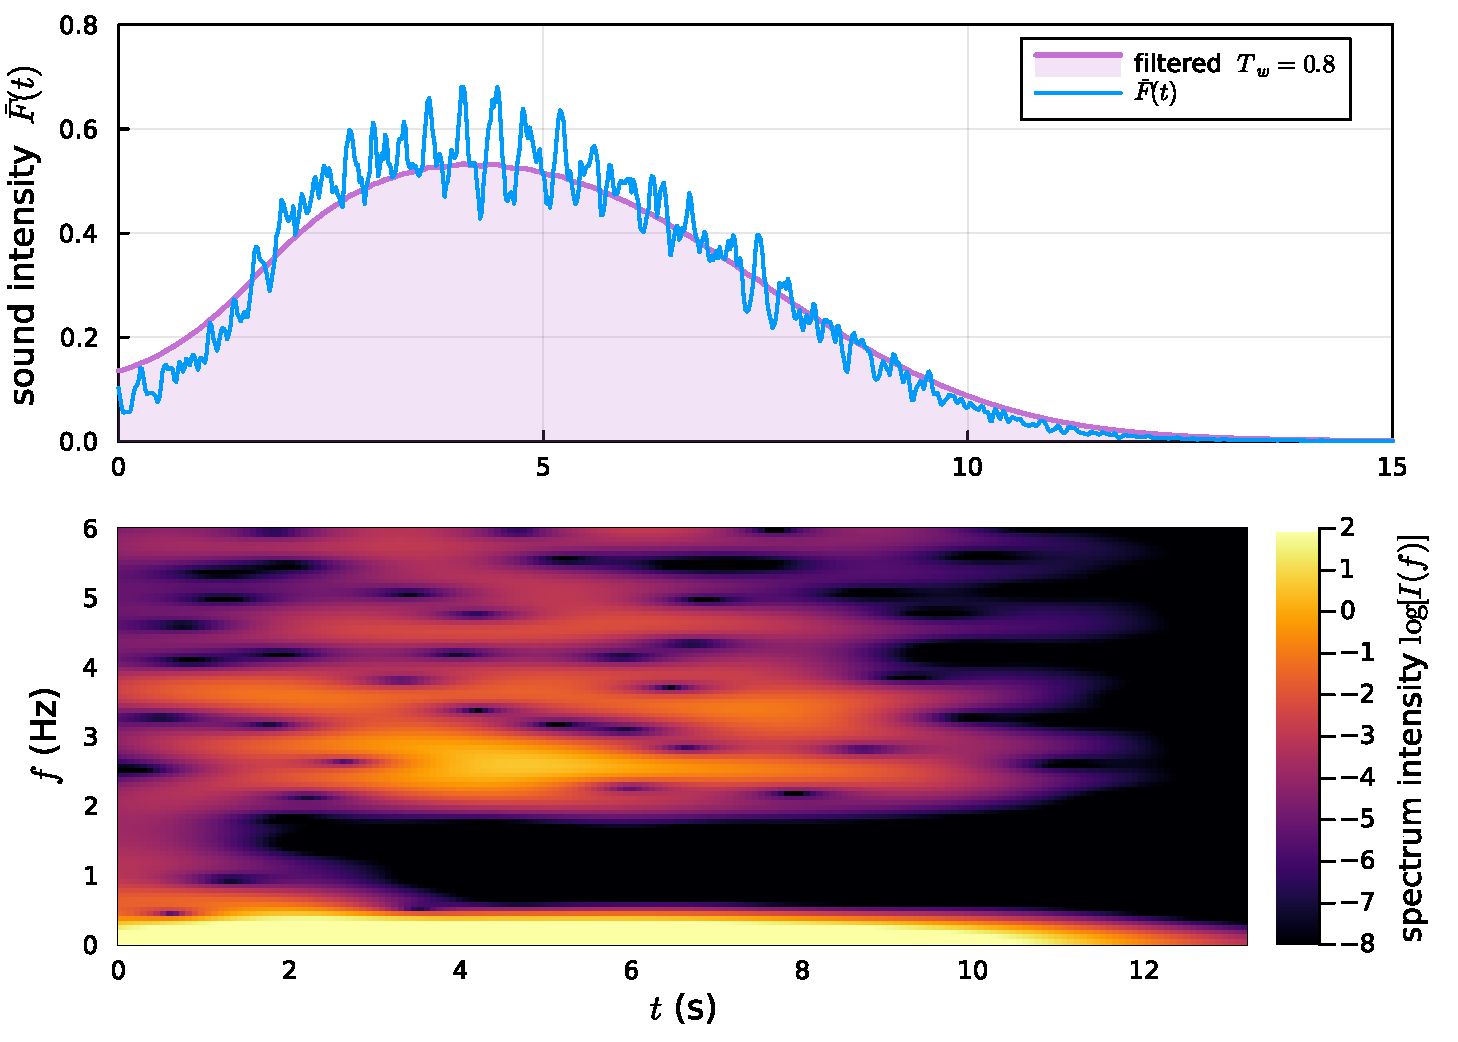
\includegraphics[width=0.9\textwidth]{sigma03typical.pdf}
    \caption{The sound intensity evolution and its time-frequency spectrum, $σ_0 = 0.3$, $η_0=0.5$.}
    \label{fig:typicalcase}
\end{figure}

It can be observed that the sound intensity initially rises and reaches its peak at around 4 seconds, followed by an exponential decay. The decay rate roughly matches the originally specified attenuation coefficient $1/τ_j$. Additionally, it is noticeable that the sound intensity curve is not smooth. Therefore, we applied a sliding average with a window width of $0.8\,\mathrm{s}$, resulting in a smoother curve. This curve closely resembles the predicted results of the SIR model.

Regarding the spectrogram, the frequency distribution of the signals at different time points broadens above 2 Hz, without any prominent patterns, although there is slightly higher intensity around the central frequency of 3 Hz. As the intensity decays, all frequency components decay as well.

\subsection{Threshold Effect}

We may tune initial applausing ratio $η_0=0.15$, which means that now there is only $15\%$ people applausing at first.

\begin{figure}[H]
    \centering
    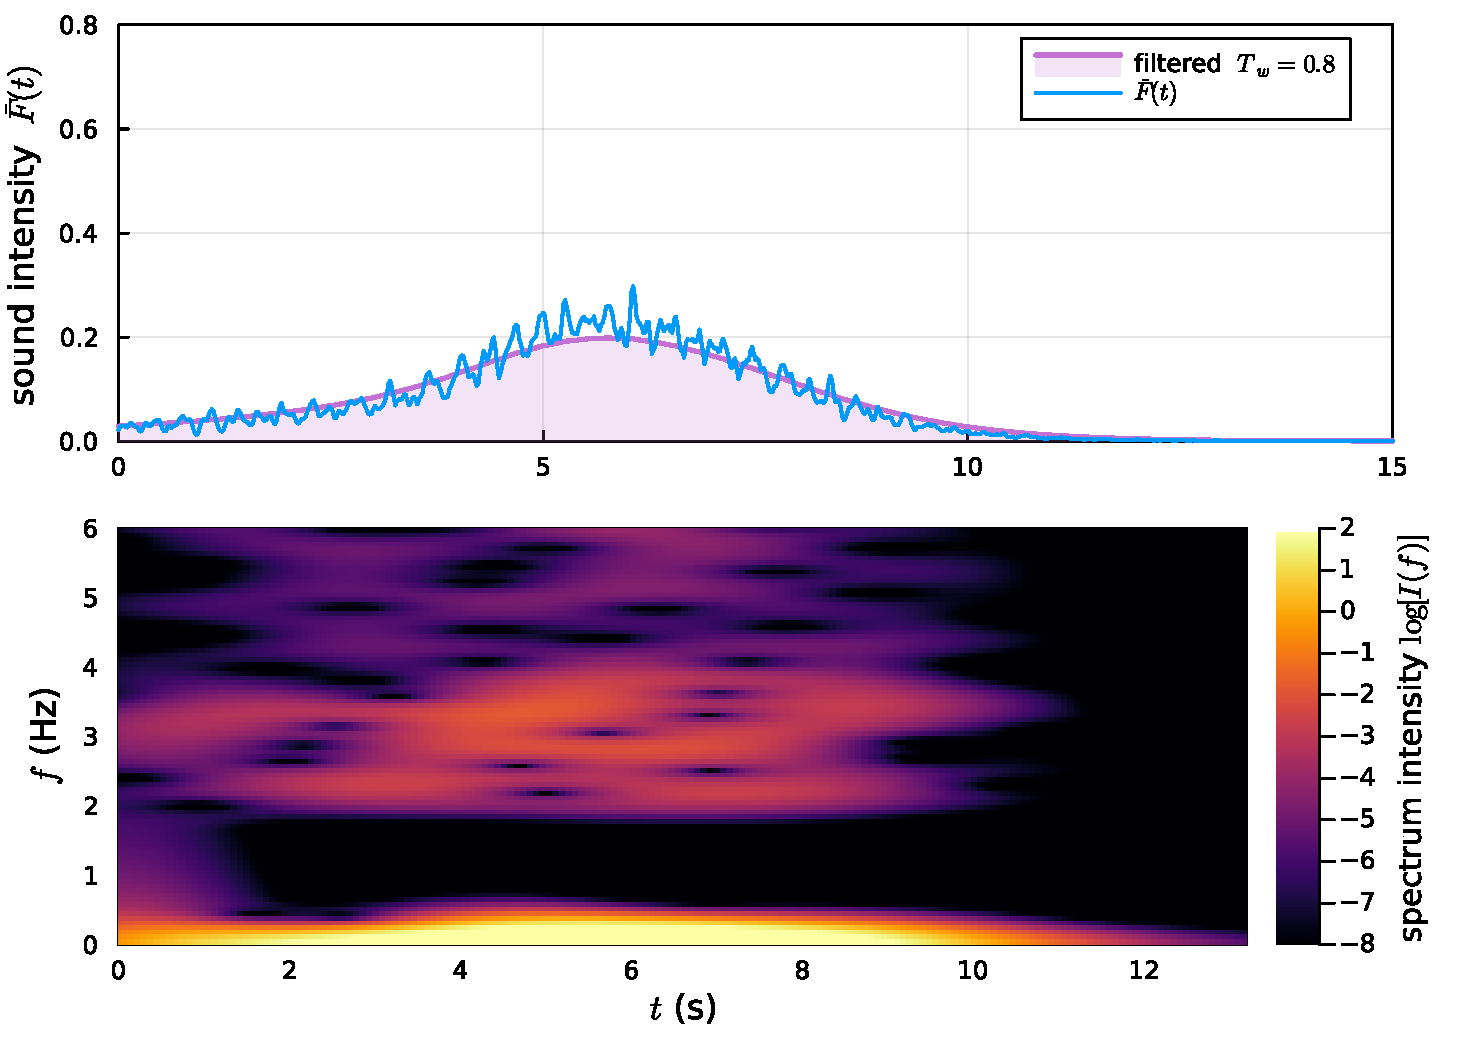
\includegraphics[width=0.9\textwidth]{eta01.pdf}
    \caption{The sound intensity evolution and its time-frequency spectrum, $σ_0 = 0.3$, $η_0=0.15$.}
    \label{fig:etalow}
\end{figure}

As shown in Fig.\ref{fig:etalow}, if the initial number of applauders is too low, it fails to establish an effective positive feedback mechanism to drive the remaining individuals to applaud, resulting in a significant decline in the peak intensity of the applause.

After multiple attempts, we discovered that the initial proportion threshold for eliciting a strong applause from the audience lies between $η_c\sim 0.1-0.2$. This implies that a minimum of 10\%-20\% of the spectators must initiate applause from the outset to achieve a collective response of applause throughout the entire venue.

\begin{figure}[H]
    \centering
    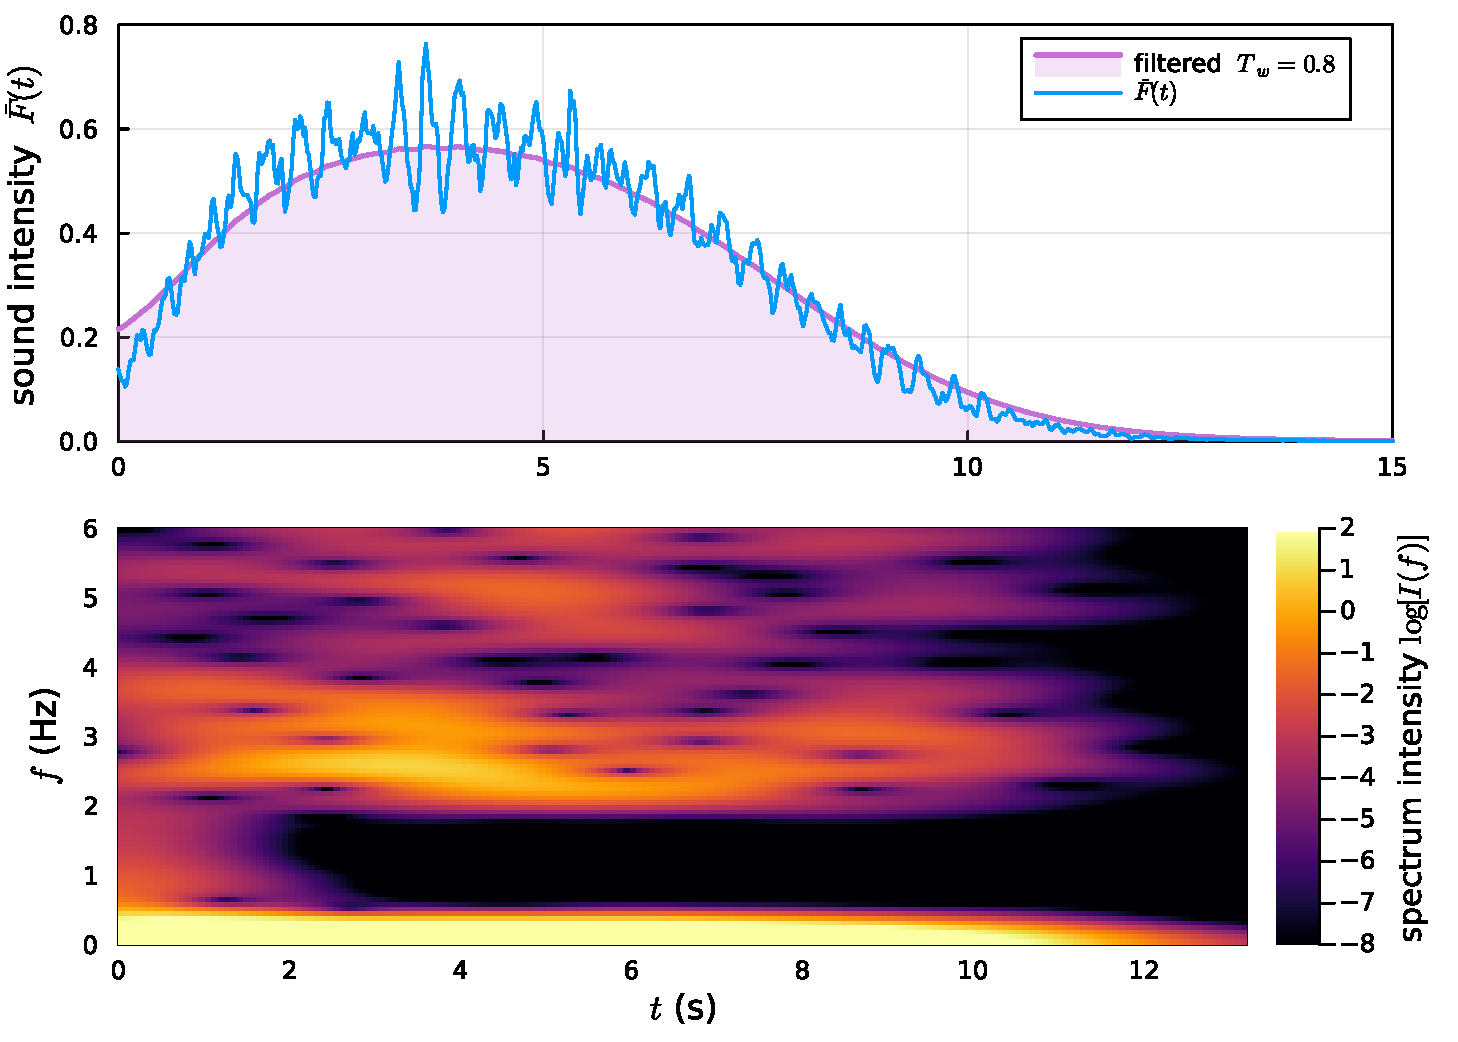
\includegraphics[width=0.9\textwidth]{eta08.pdf}
    \caption{The sound intensity evolution and its time-frequency spectrum, $σ_0 = 0.3$, $η_0=0.15$.}
    \label{fig:etahigh}
\end{figure}

In contrast, increasing the initial number of applauding individuals to $η_0 = 0.8$ does not significantly enhance the overall magnitude of applause in the auditorium, as each person's applause intensity is limited. However, elevating the initial count does contribute to a certain extent in reducing the time it takes for the applause to reach its peak, as shown in Fig.\ref{fig:etahigh}.

\subsection{Synchronization}

Homogeneity can lead to synchronization. By setting $σ_0 = 0.15$ we encounter the synchronization of applause.

\begin{figure}[H]
    \centering
    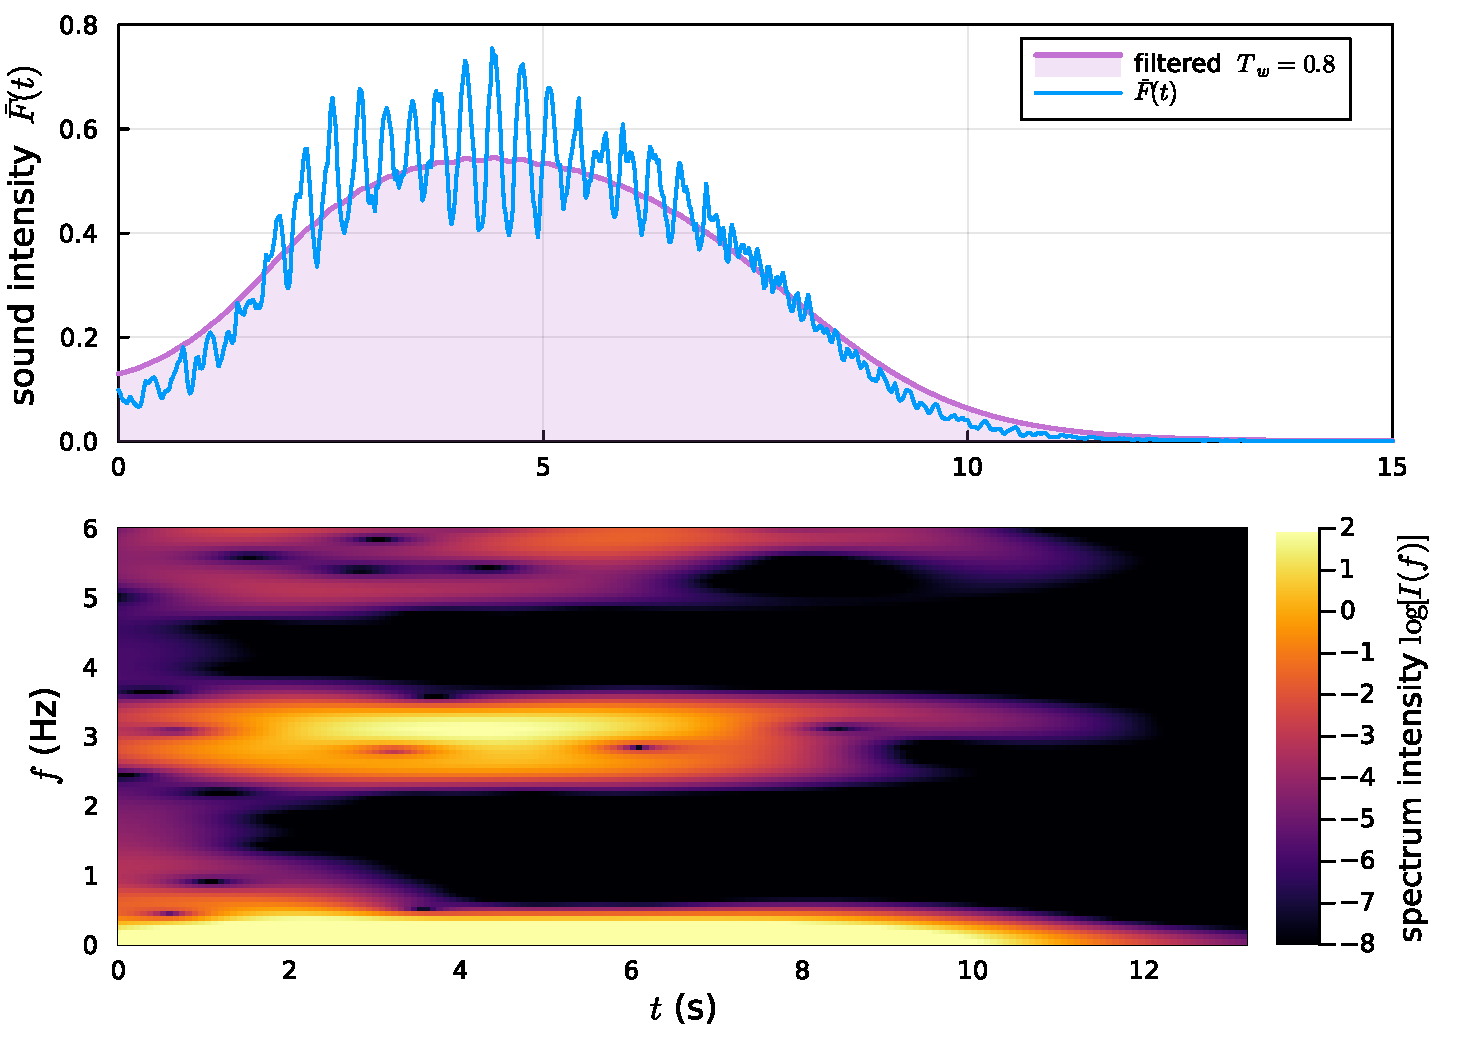
\includegraphics[width=0.9\textwidth]{sync.pdf}
    \caption{The sound intensity evolution and its time-frequency spectrum, $σ_0 = 0.15$, $η_0=0.5$. $σ_0$ is smaller than the typical case.}
    \label{fig:sync}
\end{figure}

As shown in Fig.\ref{fig:sync}, the filtered sound intensity curve exhibits no apparent differences compared to the typical case. However, a noticeable synchronization phenomenon occurs near the peak plateau. This phenomenon can be further confirmed in the time-frequency spectrum, where a distinct peak is observed around 3Hz. Moreover, the duration of this peak aligns with the duration of synchronous oscillations in the time-domain signal.

On the other hand, the synchronization can also be obtained by increasing the coupling. According to the theory of Kuramoto\footnote{Our model is different, however the analytical solution seems impossible so we adopt Kuramoto model.}, the critical coupling for the typical case $σ_0 = 0.3$ is
\begin{equation}
    κ_c = \sqrt{\frac{2}{π^3}} \bar{ω} σ_0 ≈ 1.43 \,\mathrm{s^{-1}}
\end{equation}
However in our model the value is much larger. For $σ=0.3$, we numerically estimate that
\begin{equation}
    κ_c ≈ 5 \, \mathrm{s^{-1}}
\end{equation}

And we present the simulation result for $\bar{κ}=5.3$ in Fig.\ref{fig:synckappa}.

\begin{figure}[H]
    \centering
    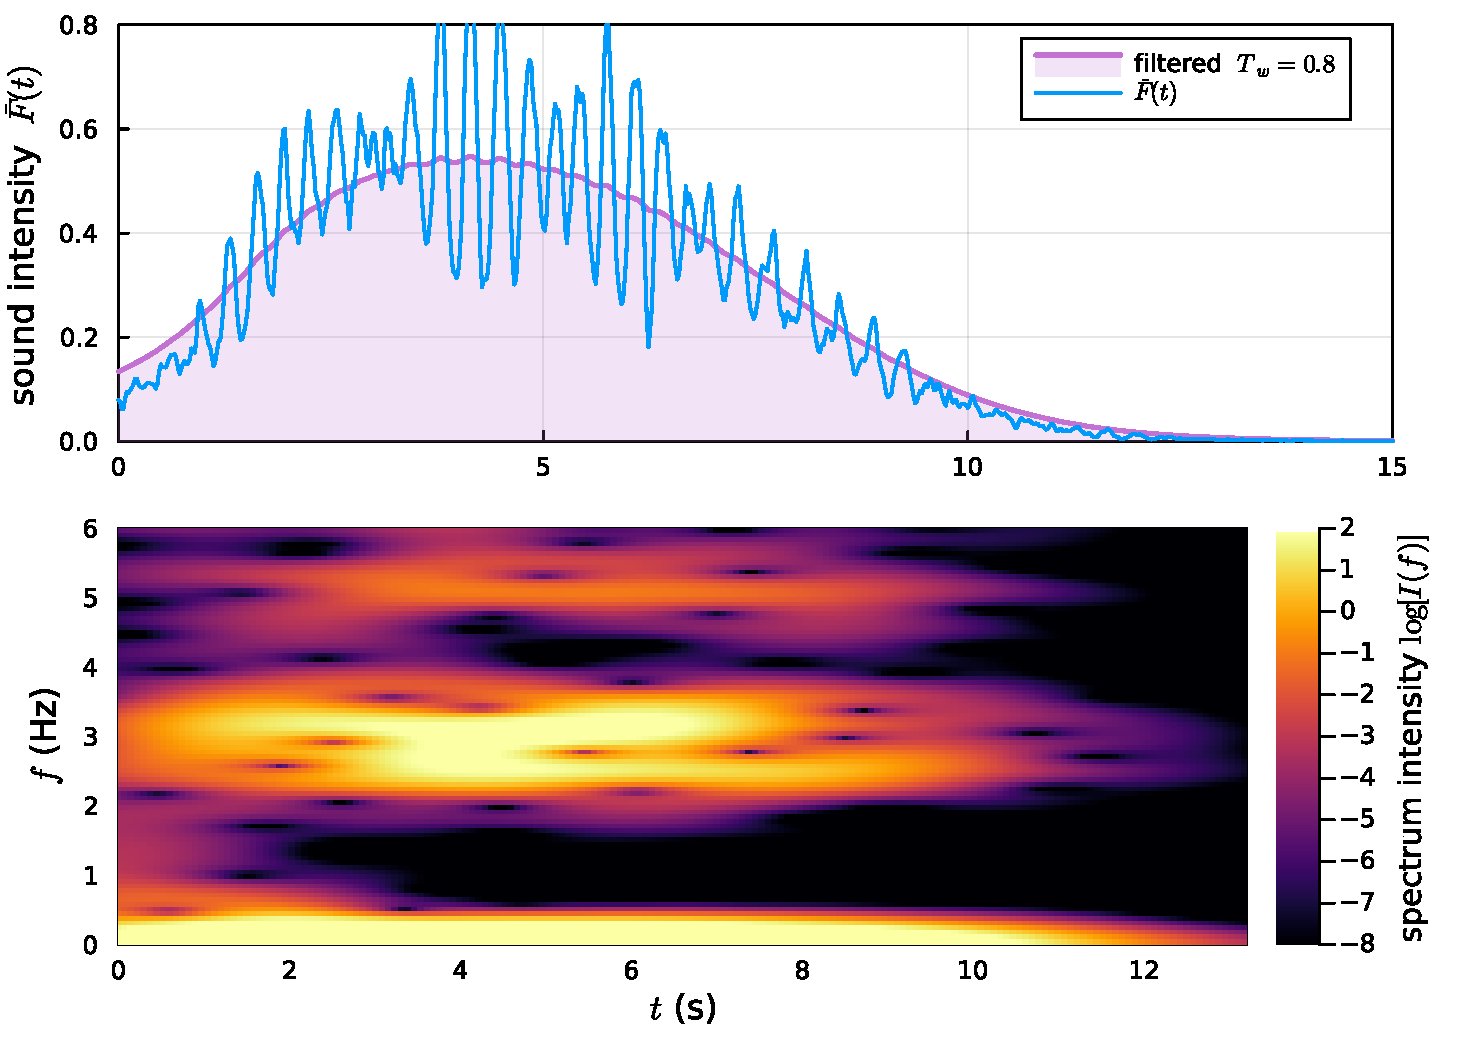
\includegraphics[width=0.9\textwidth]{k53.pdf}
    \caption{The sound intensity evolution and its time-frequency spectrum, $σ_0 = 0.3$, $η_0=0.5$. $\bar{κ} = 5.3$ is higher than the typical case $\bar{κ} = 2.0$.}
    \label{fig:synckappa}
\end{figure}

It can be observed that, \textbf{although the time pattern is similar to Fig.\ref{fig:sync}, the spectrum looks different!}. 

In \textbf{homogeneity} leading synchronization ($σ_0$ is low), the spectrum is more centralized, with clear background. While in \textbf{stong coupling} leading synchronization, the spectrum shows a broad plateau around the center frequency, and the background is not so flat (in other words, more ``dirty''). This discovery is likely to be confirmed in experiments.

\section{Summary \& Outlook}

\subsection{Advantages of the Model}

Our model possesses the following advantages:
\begin{enumerate}
    \item In terms of sound intensity, our model's simulation results closely align with the predicted sound intensity of the SIR model.

    \item Regarding synchronous phenomena, our model shares similarities with Kuramoto's model as it also predicts synchronization phenomena.

    \item Our model exhibits strong scalability, allowing for easy incorporation of new parameters by simply adding or modifying different terms in the CMT equations. For instance, if spatial configurations are to be considered, introducing neighboring coupling terms would suffice.
\end{enumerate}


\subsection{Limitations of the Model}

The CMT model itself is very scalable, but the key is to make each parameter meaningful. The limitations are
\begin{enumerate}
    \item The model assume the expectated applausing time of an individual with the absence of the environment to be a constant. This is of course not the real case.
    \item The model neglected the spatial information.
    \item The reverberation effect is not included in the mean-field term.
\end{enumerate}

\subsection{Findings}

\begin{itemize}
    \item \textbf{Threshold effect:} There is a threshold for the whole crowd to start applausing. If the number initial applausing spectators is small, the crowd is unlikely to burst into applausing. However, when this ratio exceeds another threshold, the final sound intensity will reach saturation, and the influence of initial conditions becomes less pronounced.
    \item \textbf{Synchronization phenomena:} The phenomenon of synchronization can be understood as a competition between heterogeneity and coupling strength. This is not novel, since it is explained in existing investigations.
    
    The unique finding of our work is that, synchronization arising from strong coupling and low heterogeneity exhibits similarities in the temporal domain of signals, but differs in spectral information. Even the coupling is larger and the system is in synchronization, the heterogeneity of intrinsic parameters can be observed in the time-frequency spectrum.
\end{itemize}

\subsection{Further Problems}

Further research areas of interest include:

\begin{itemize}
\item Investigating the potential impact of the environment on individual patience, specifically examining whether $τ_j$ is influenced by mean-field effects. This may characterizing the extending of applause duration.

\item Exploring the specific mechanisms of synchronization observed in experiments. That is determining whether the synchronization is due to enhanced homogeneity within the crowd or to increased coupling between individuals.

\item Developing a quantitative measure for the coupling coefficients $κ$ in real-world settings.
\end{itemize}

\section{Appendix}
\subsection{Logistic Function}

We have extensively utilized the Logistic function in our modeling, therefore it is necessary to provide a brief introduction to it.

The logistic function is a mathematical function that maps input values to a range between 0 and 1. It is often used to model population growth, probability, and other phenomena that exhibit sigmoidal behavior. The logistic function is defined by the formula:
\begin{equation}
    l(x) = \frac{1}{1+e^{-x}},
\end{equation}
As x approaches positive infinity, the logistic function asymptotically approaches 1, while as x approaches negative infinity, it asymptotically approaches 0. It is commonly used in various fields such as statistics, biology, economics, and neural networks. In out modeling, we use a logistic function with a transition time parameter $τ_0$, which reads:
\begin{equation}
    l(x-x_0) = \frac{1}{1+\exp\left( -\frac{x-x_0}{τ_0} \right)},
\end{equation}

\subsection{Software Dependencies \& Code Access}

Coding work of this course research is completed using the \ic{Julia} language \cite{julialang}.

The project highly relies on the package \ic{DifferentialEquations.jl} \cite{DifferentialEquations}, which provides generic interfaces for numerically solving differential equations, especially ODEs and dynamical systems.

The report document, \LaTeX source code, programs and figures can all be found in \textcolor{blue}{\href{https://github.com/PDE2718/NaiveSDE.jl}{the author's Github repository}}.

\newpage
\printbibliography





% \forcednewpage



% \section{aaa}
% 你好,world!

% \begin{equation}
%     \left⟨ \cos{α} \frac{𝐀}{Γ}π \right⟩    
% \end{equation}

% \begin{equation}
%     iℏ \frac{d}{dt} ψ = H ψ
% \end{equation}



% bb

% cc

% \ic{some code}

\end{document}

